\chapter{The \chips R\&D Project}
\label{chap:chips}

\section{Things to talk about}

- General overview of why a large, cheap detector like CHIPS is needed
PLOT:
- Brief overview of what CHIPS could add to physics, what it can detect etc...
- general non-detailed description of the general principles behind CHIPS

REF: Hyper-k letter of intent~\cite{abe2011}
REF: Dune CDR~\cite{acciarri2016}

- First how beam water Cherenkov detect events
- Describe the Numi beam
- An aside on the off-axis effect
- Describe the Cherenkov effect
- Describe the flux and expected cross-sections / types of event
- Give the expected number of events that CHIPS should see
- An aside on GENIE which we used for event generation
- Describe all the possible interactions that can be observed in CHIPS
- What are the classic difficulties with water Cherenkov detectors
- Brief description of how PMTs detect the cherenkov light
- CHIPS detector simulation
- Example plots of events for different signature types of events...

- The CHIPS-M detector and conclusions

- The CHIPS-10 detector
- General structure, how it all holds together
- How it is deployed/extended
- How it detects the Cherenkov light with PMTs arranged in planes
- How the construction went
- Current status and future plans

- The tau neutrino component is negligible and not predicted by the simulation

\section{Diagrams}

\begin{figure}
    \includegraphics[width=0.8\textwidth]{diagrams/4-chips/sunrise.jpeg}
    \caption[Sunrise over the \chips detector.]
    {Sunrise over the \chips detector structure. The perfectly calm pit water
        produces the mirror effect.}
    \label{fig:sunrise}
\end{figure}

\begin{figure}
    \includegraphics[width=0.8\textwidth]{diagrams/4-chips/from_the_sky.jpg}
    \caption[Picture of the \chips detector from the air.]
    {Picture of the \chips detector taken from an airplane. The Wentworth 2W pit is in the lower
        half of the image, with the half built detector, huts and construction containers visable.}
    \label{fig:from_the_sky}
\end{figure}

\begin{figure}
    \includegraphics[width=0.8\textwidth]{diagrams/4-chips/location.png}
    \caption[Satellite view of the Wentworth 2W mine pit.]
    {Satellite view of the Wentworth 2W mine pit in northern Minnesota.
        The size markers are shown for scale. Image taken from Ref.\cite{adamson2013}.}
    \label{fig:location}
\end{figure}

\begin{figure}
    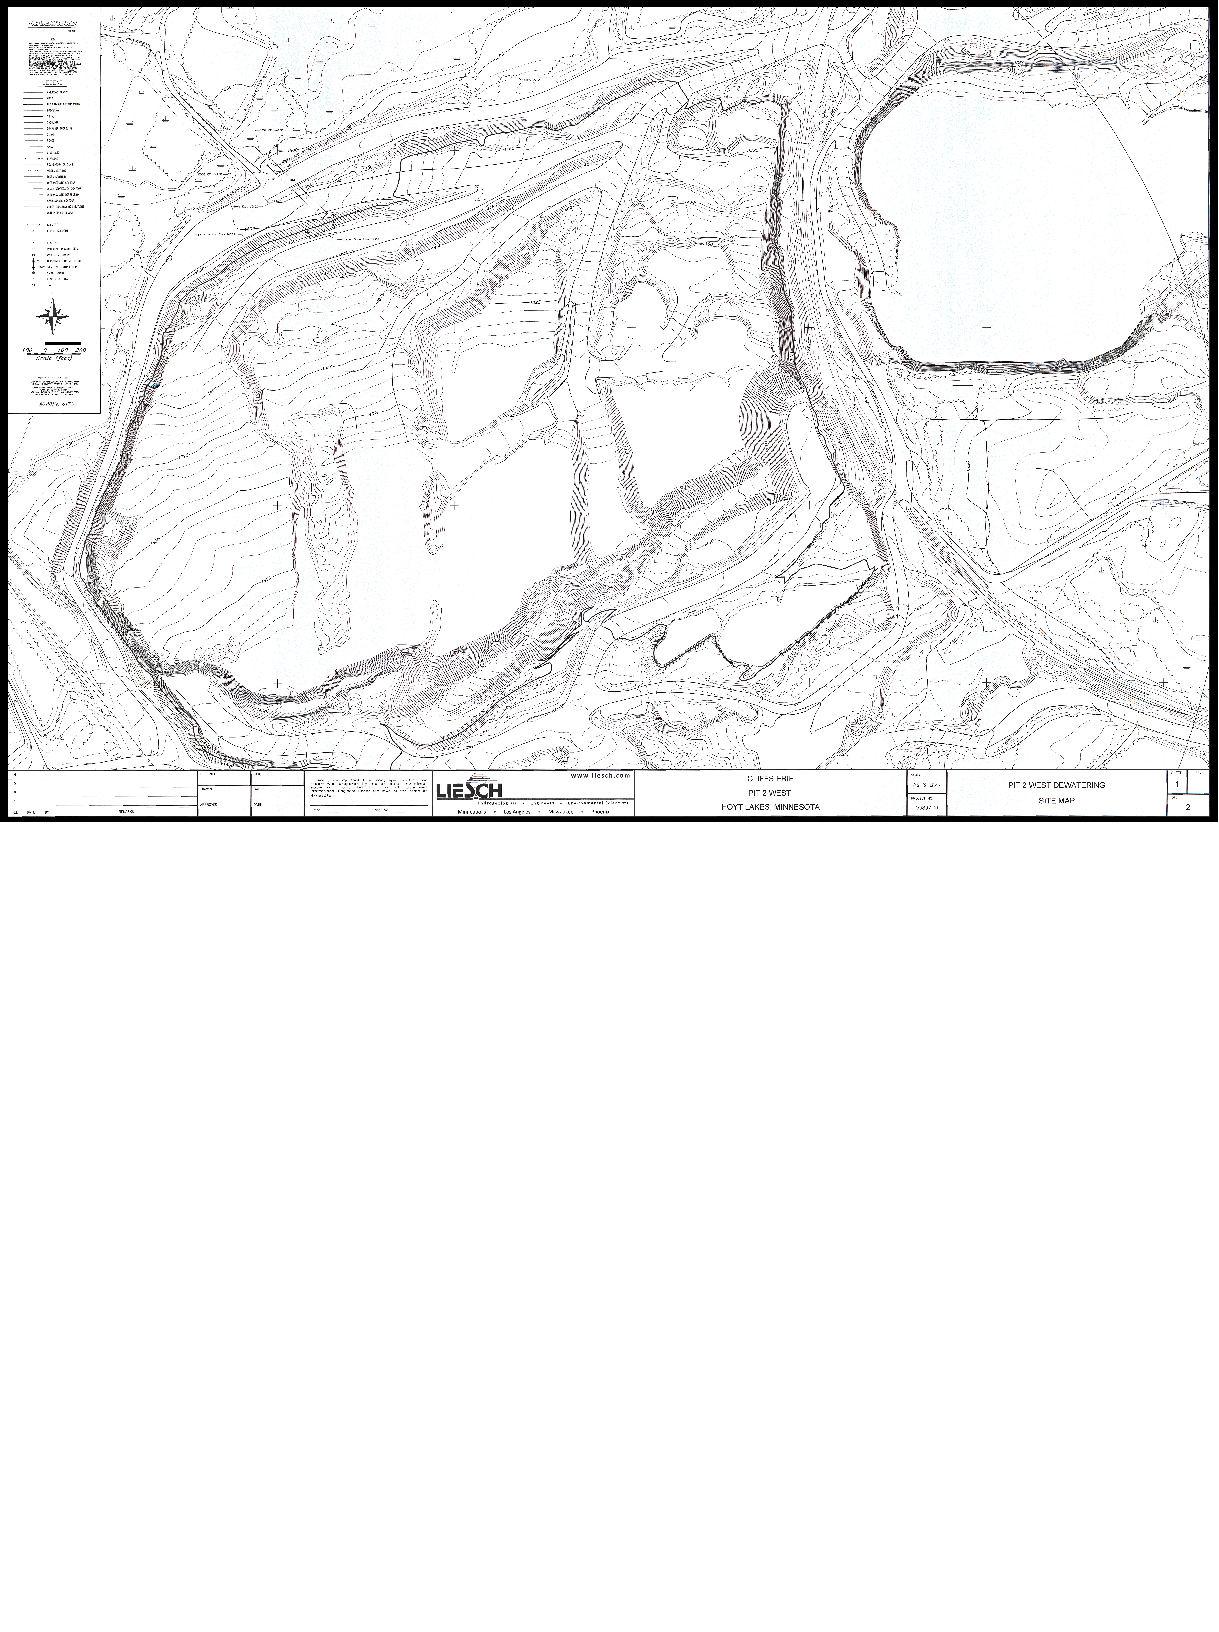
\includegraphics[width=0.8\textwidth]{diagrams/4-chips/contour_map.pdf}
    \caption[Topographic map of the Wentworth 2W mine pit.]
    {Topographic map of the Wentworth 2W mine pit. The contours are given in intervals of 5 feet,
        with the central areas of the pit having a depth of 50m. Image taken from Ref.\cite{adamson2013}.}
    \label{fig:contour_map}
\end{figure}

\begin{figure}
    \includegraphics[width=0.8\textwidth]{diagrams/4-chips/chips_m.png}
    \caption[Picture of the \chipsm detector.]
    {Picture of the \chipsm detector just before deployment. The umbilical is visable, attached to the
        bottom endcap of the detector.}
    \label{fig:chips_m}
\end{figure}

\begin{figure}
    \includegraphics[width=0.8\textwidth]{diagrams/4-chips/chips_render_1.png}
    \caption[Graphical rendering of the \chipsfive detector with liner cutaway.]
    {Graphical rendering of the \chipsfive detector with a section of the liner cutaway.
        The bottom endcap and wall planes are visable,
        as well as the top endcap structure and floatation.}
    \label{fig:chips_render_1}
\end{figure}

\begin{figure}
    \includegraphics[width=0.8\textwidth]{diagrams/4-chips/chips_render_2.png}
    \caption[Graphical rendering of the \chipsfive detector structure.]
    {Graphical rendering of the \chipsfive detector structure.}
    \label{fig:chips_render_2}
\end{figure}

\begin{figure}
    \includegraphics[width=0.8\textwidth]{diagrams/4-chips/numi_map.png}
    \caption[Map of detector locations in the \numi beam.]
    {Map of the \chips, \nova and \minos locations in the \numi beam showing the expected
        neutrino event rates, assuming no oscillations. Lines of constant L/E are shown by the contours.
        Image taken from Ref.\cite{adamson2013}.}
    \label{fig:numi_map}
\end{figure}

\begin{figure}
    \includegraphics[width=\textwidth]{diagrams/4-chips/numi_beam.png}
    \caption[Schematic of the \numi beam.]
    {Schematic of the main components of the \numi beam (not to scale) shown with their dimensions.
        The horns control if the beam is in neutrino or anti-neutrino mode. Image taken from Ref.\cite{adamson2016}.}
    \label{fig:numi_beam}
\end{figure}

\begin{figure}
    \includegraphics[width=0.8\textwidth]{diagrams/4-chips/numi_axis.png}
    \caption[Neutrino flux for different detectors in the \numi beam.]
    {Neutrino flux for different detectors in the \numi beam.
        The difference is caused by the different off-axis angles.
        Image taken from Ref.\cite{adamson2013}.}
    \label{fig:numi_axis}
\end{figure}

\begin{figure}
    \includegraphics[width=0.8\textwidth]{diagrams/4-chips/flux.png}
    \caption[flux short]
    {}
    \label{fig:flux}
\end{figure}

\begin{figure}
    \includegraphics[width=0.8\textwidth]{diagrams/4-chips/xsec_cc_nu_e_O16.png}
    \caption[xsec cc nu e O16 short]
    {xsec cc nu e O16 long}
    \label{fig:xsec_cc_nu_e_O16}
\end{figure}

\begin{figure}
    \includegraphics[width=\textwidth]{diagrams/4-chips/sim_event.png}
    \caption[sim event short]
    {sim event long}
    \label{fig:sim_event}
\end{figure}

\begin{figure}
    \includegraphics[width=0.8\textwidth]{diagrams/4-chips/cosmics.png}
    \caption[cosmics short]
    {cosmics long}
    \label{fig:cosmics}
\end{figure}

- POM diagram
- Cosmic rate given the water overburden diagram
- CHIPS fiducial volume diagram with dimensions around the sides
- CHIPS expected event rate plot with and without oscillations
- Cherenkov effect diagram
- Floating dock diagram
- Deployment diagram

\section{References}

- CHIPS letter of intent~\cite{adamson2013}
- CHIPS attenuation length paper~\cite{amat2017}
- CHIPS reco paper~\cite{blake2016}
- Karol prospects for CHIPS paper~\cite{lang2015}
- Andy CHIPS-M prototype construction and simulations~\cite{perch2015}
- Maciej prototype detection unit~\cite{pfutznerProto2017}
- Sensitivity Determination in the CHIPS Neutrino Detector~\cite{adde2016}
- The Numi beam big paper~\cite{adamson2016}
- Icecube DOM paper
- km3net General paper
- Km3net optical module paper
- Nemo-3 PMT paper

\section{Reference notes}

